%----------------------------------------------------------------------------------------
%	PACKAGES AND OTHER DOCUMENT CONFIGURATIONS
%------------------------------------------------------------------------
\documentclass[11pt]{article}
\usepackage[utf8]{inputenc} % Required for inputting international characters
\usepackage[T1]{fontenc} % Output font encoding for international characters
\usepackage{mathpazo} % Palatino font
\usepackage[czech]{babel} % Czech
\usepackage{graphicx}  % Graphics
\usepackage{amsmath}
\usepackage{pdfpages}

\begin{document}
	
	%----------------------------------------------------------------------------------------
	%	TITLE PAGE
	%----------------------------------------------------------------------------------------
	
	\begin{titlepage} % Suppresses displaying the page number on the title page and the subsequent page counts as page 1
		\newcommand{\HRule}{\rule{\linewidth}{0.5mm}} % Defines a new command for horizontal lines, change thickness here
		
		\center % Centre everything on the page
		
		%------------------------------------------------
		%	Headings
		%------------------------------------------------
		
		\textsc{\LARGE České vysoké učení technické v Praze}\\[1.5cm] % Main heading such as the name of your university/college
		
		\textsc{\Large Algoritmy digitální kartografie a GIS}\\[0.5cm] % Major heading such as course name
		
		\textsc{\large Katedra geomatiky}\\[0.5cm] % Minor heading such as course title
		
		%------------------------------------------------
		%	Title
		%------------------------------------------------
		
		\HRule\\[0.4cm]
		
		{\huge\bfseries Úloha č. 2: Konvexní obálky}\\[0.4cm] % Title of your document
		
		\HRule\\[1.5cm]
		
		%------------------------------------------------
		%	Author(s)
		%------------------------------------------------
		
		
		
		
		% If you don't want a supervisor, uncomment the two lines below and comment the code above
		Monika \textsc{Křížová} % Your name
		
		Marek \textsc{Hoffmann}
		
		%------------------------------------------------
		%	Date
		%------------------------------------------------
		
		\vfill\vfill\vfill % Position the date 3/4 down the remaining page
		
		{\large 06.11.2021} % Date, change the \today to a set date if you want to be precise
		
		%------------------------------------------------
		%	Logo
		%------------------------------------------------
		
		%\vfill\vfill
		%\includegraphics[width=0.2\textwidth]{placeholder.jpg}\\[1cm] % Include a department/university logo - this will require the graphicx package
		
		%----------------------------------------------------------------------------------------
		
		\vfill % Push the date up 1/4 of the remaining page
		
	\end{titlepage}
	
	%----------------------------------------------------------------------------------------
	
	
	%----------------------------------------------------------------------------------------
	%	TABLE OF CONTENT
	%----------------------------------------------------------------------------------------
	
	\tableofcontents
	%\thispagestyle{empty}
	
	\clearpage
	
	%----------------------------------------------------------------------------------------
	%	ZADÁNÍ
	%----------------------------------------------------------------------------------------
	
	\section{Zadání}
	Vytvořte aplikaci s grafickým uživatelským rozhraním, která bude ze souboru načítat polygony budov a následně je bude generalizovat na obdélníky s plochou odpovídající generalizované budově a bude vytvářet konvexní obálky. Hlavní směry budov budou určeny metodami Minimum Area Enclosing Rectangle a Wall Average.
	
	Přesné zadání je vloženo na následující stranu.
	
	
	
	
	%---------------------------------------------------------------------
	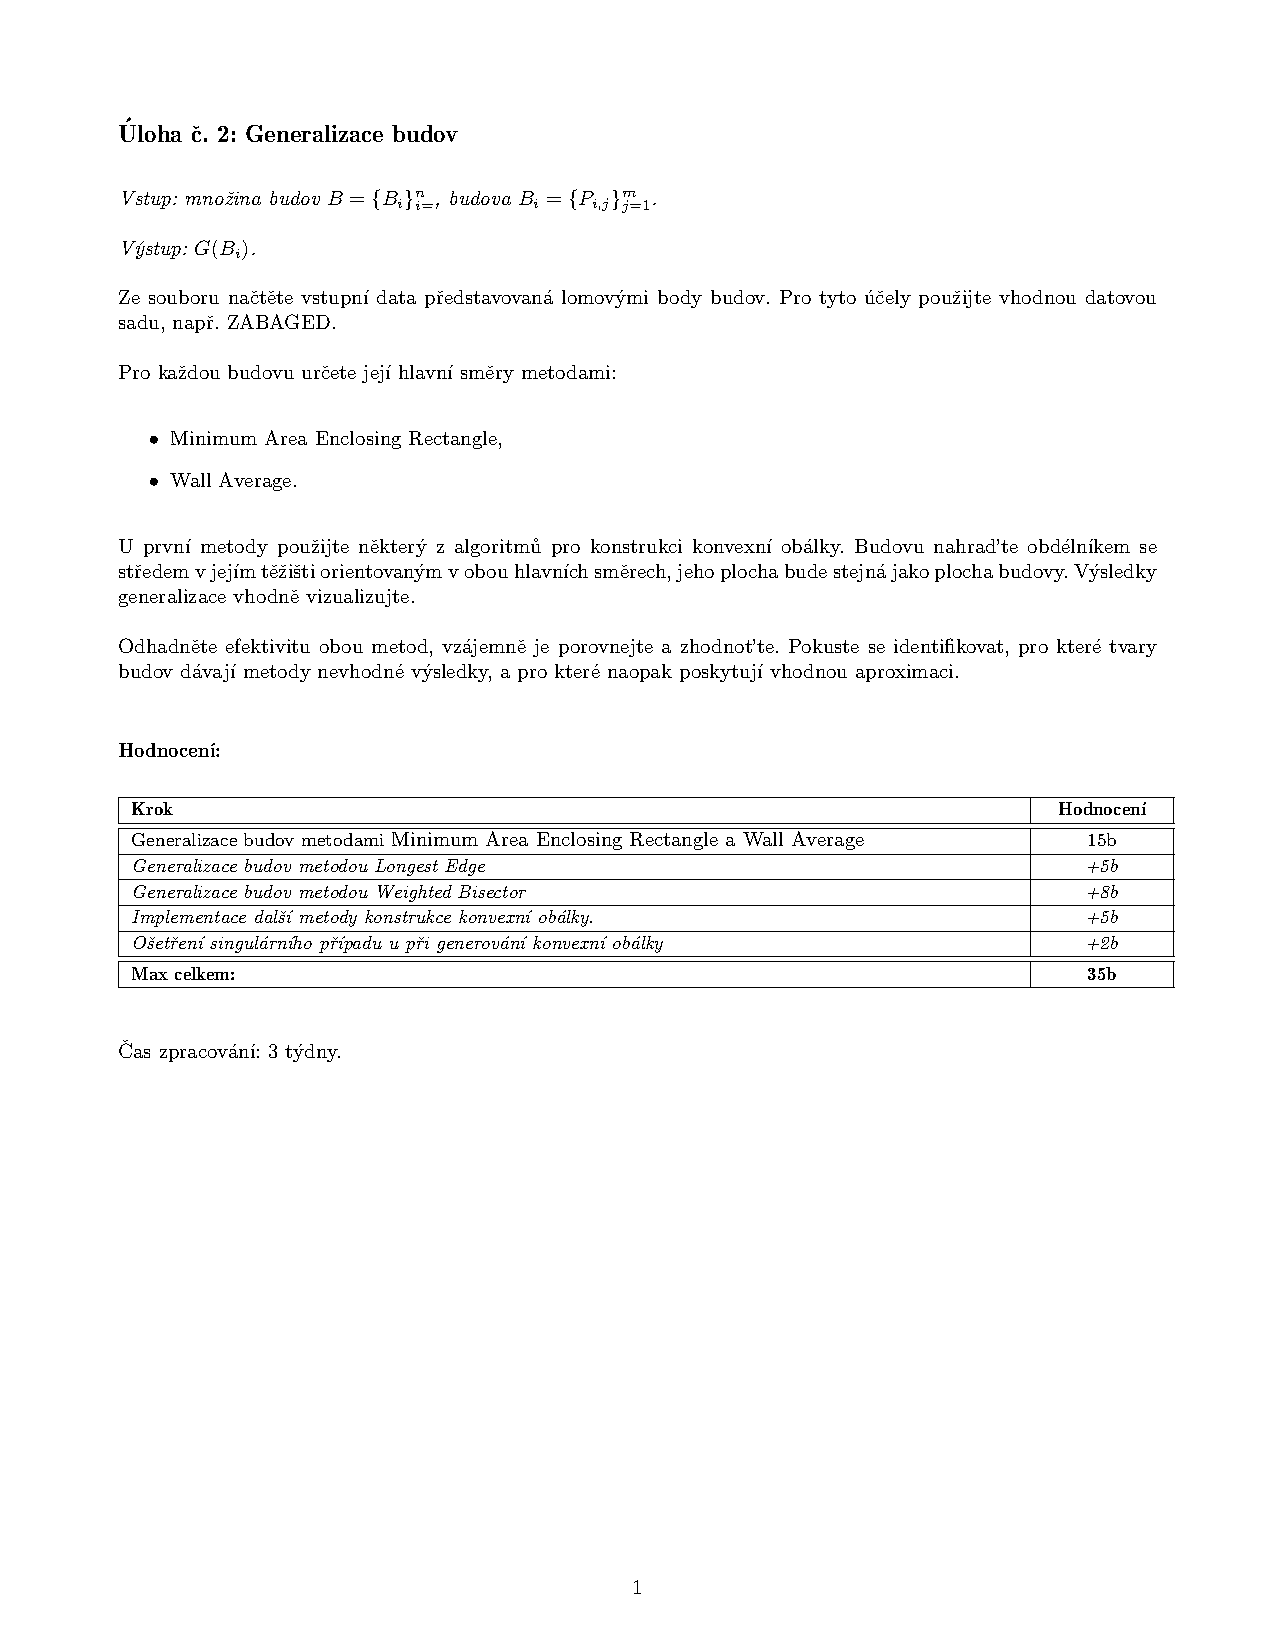
\includepdf{adkcv2.pdf}
	
	
	
	%---------------------------------------------------------------------
	
	%----------------------------------------------------------------------------------------
	%	ÚDAJE O BONUSOVÝCH ÚLOHÁCH
	%----------------------------------------------------------------------------------------
	
	\section{Údaje o bonusových úlohách}
	Zpracovány byly celkem 3 bonusové úlohy ze 4 zadaných.
	
	\begin{itemize}
		\item Generalizace budov metodou Longest Edge +5b
		\item Generalizace budov metodou Weighted Bisector +8b
		\item Implementace další metody konstrukce konvexní obálky. +5b
	\end{itemize}
	
	Generalizace budov metodou Longest Edge byla implementována ve třídě Algorithms, je možné ji spustit pomocí tlačítka Building simplify po předchozím výběru v comboBoxu umožňujícího výběr metody generalizace polygonu.
	
	Generalizace budov metodou Weighted Bisector byla stejně jako metoda Longest Edge implementována ve třídě Algorithms a taktéž je ji možné spustit pomocí tlačítka Building simplify po předchozím výběru v comboBoxu umožňujícího výběr metody generalizace polygonu.
	
	Pro implementaci další metody konstrukce konvexní obálky byla vybrána metoda Quick Hull, jež byla přidána do třídy Algorithms. Pro její spuštění je nutné vybrat tuto metodu v náležitém comboBoxu a následně stisknout tlačítko Create convex hull.
	
	
	%----------------------------------------------------------------------------------------
	%	POPIS PROBLÉMU
	%----------------------------------------------------------------------------------------
	
	\section{Popis problému}
	Generalizace je v kartografii velmi důležitý proces, který je používán například při změně měřítka mapy, změně jejího účelu nebo pro zlepšení grafické přehlednosti. Generalizace může být provedena několika různými metodami, v řešené úloze byla aplikována tzv. geometrická generalizace, jež spočívá ve zjednodušení tvaru objektu. Objekty (v této úloze budovy) byly generalizovány na obdélníky s plochou odpovídající ploše původních objektů.
	
	Jednotlivé generalizační algoritmy hledají hlavní směr natočení budovy, po nalezení tohoto směru se vytvoří opsaný obdélník s minimálním obsahem, jež je natočený do tohoto směru (dále pod zkratkou MMB). MMB se následně zmenší tak, aby byla jeho plocha totožná s plochou generalizovaného objektu. 
	
	%----------------------------------------------------------------------------------------
	%	POPIS ALGORITMŮ
	%----------------------------------------------------------------------------------------
	
	\section{Popisy algoritmů}
	\subsection{Tvorba konvexní obálky}
	\subsubsection{Jarvis scan}
	
	Prvním krokem při tvorbě konvexní obálky $\mathcal{H}$ metodou Jarvis scan je nalezení pivotu \textit{q}. Tento bod je bod s nejmenší souřadnicí \textit{y} v množině bodů \textit{S}. Dalším krokem je nalezení bodu \textit{p}, jež svírá největší úhel s rovnoběžkou s osou \textit{x} procházející bodem \textit{q}. Nalezený bod se přidá do $\mathcal{H}$ a opět se hledá bod, jež bude svírat s předchozím bodem největší úhel. Tímto způsobem se do $\mathcal{H}$ přidávají body do okamžiku, kdy by byl přidávaným bodem bod \textit{q}. Tato metoda je velmi jednouchá, ale kvůli časové náročnosti nevhodná pro velké množiny bodů.
	
	\subsubsection{Quick Hull}
	
	V algoritmu Quick Hull je nejprve nutné seřadit množinu bodů \textit{S} podle souřadnice \textit{x} a následně ze setříděného souboru vybrat dva body, tzv. pivoty. Bod \textit{$ q_{1} $} je bodem s nejmenší souřadnicí \textit{x}, bod \textit{$ q_3 $} má naopak souřadnici x ze souboru bodů \textit{S} největší. Konvexní obálka $\mathcal{H}$ se vytváří ze dvou částí – horní ($\mathcal{H_U}$) a spodní $\mathcal{H_L}$ konvexní obálky. 
	Do $\mathcal{H_U}$ se přidávají body ležící nalevo od spojnice pivotů \textit{$ q_{1} $} a \textit{$ q_{3} $}, do $\mathcal{H_L}$ naopak body ležící na pravé straně od spojnice týchž bodů.
	
	Posledním krokem je spojení obou částí konvexní obálky do výsledné množiny $\mathcal{H}$. Nejprve se do $\mathcal{H}$ přidá bod \textit{$ q_3 $}, poté se provede rekurze $\mathcal{H_U}$, pomocí níž se do $\mathcal{H}$ přidají body z horní části konvexní obálky, poté se přidá bod \textit{$ q_{1} $} a posledním krokem je provedení rekurze $\mathcal{H_L}$, díky níž se do konvexní obálky přidají i body ze spodní části konvexní obálky.
	
	
	\subsection{Generalizace budov}
	\subsubsection{Minimum Enlosing Rectangle}
	Algoritmus se snaží vyhledat takovou hranu konvexní obálky $\mathcal{H}$, aby po vytvoření opsaného obdélníka s jednou stranou kolineární s touto hranou měl takto vytvořený obdélník minimální plochu.
	
	Algoritmus využívá již zkonstruovanou konvexní obálku $\mathcal{H}$, pro jejíž hrany jsou vypočítávány směrnice $\sigma$ hrany \textit{e}: 
	
	\begin{equation}
		\tan\sigma=\frac{d_x}{d_y}, 
	\end{equation}
	kde $d_{x}$ a $d_{y}$ jsou souřadnicové rozdíly počátečního a koncového bodu hrany konvexní obálky $\mathcal{H}$. Všechny body množiny \textit{S} se následně pomocí matice rotace \textit{R} otočí o úhel $-\sigma$:
	
	\begin{equation}
		S_R=R(-\sigma)S 
	\end{equation}
	
		Pro otočené body množiny se vytvoří MMB s následujícími souřadnicemi vrcholů:
		
		\begin{equation}
			V_1 = [\underline{x}, \underline{y}], V_2 = [\overline{x}, \underline{y}],
			V_3 = [\overline{x}, \overline{y}],
			V_4 = [\underline{x}, \overline{y}],
		\end{equation}
		
		kde $\underline{x},\overline{x},\underline{y}, \overline{x}$ jsou minimální a maximální souřadnice natočených bodů množiny \textit{$ S_R $}. Vypočte se plocha vytvořeného \textit{MMB}:
		
		\begin{equation}
			A = (\overline{x}-\underline{x})(\overline{y}-\underline{y}),
		\end{equation}
		
		jež se následně porovná s minimální uloženou plochou. Je-li vypočtená plocha \textit{A} menší než je plocha minimální, uloží se jako nové minimum. Dále se uloží pro tuto plochu uloží úhel $ \sigma_{min} $ a \textit{$MMB_{min}$}. Po ukončení výpočtu 
		totoho cyklu je již vypočten výsledný úhel natočení budovy $ \sigma_{min} $. Následně je nutné \textit{MMB} natočit o tento úhel a zmenšit tak, aby byla plocha \textit{MMB} rovna ploše generalizovaného polygonu. Tento postup bude používán i pro další metody.
		
		\textit{$MMB_{min}$} se otočí o úhel $ \sigma_{min} $:  
		
		\begin{equation}
		\mathcal{R} = R(\sigma_{min})MMB_{min}, 
		\end{equation}
		
		následně se jeho plocha proporcionálně zmenší vůči těžišti tak, aby byla rovna ploše generalizovaného polygonu. Nejprve je nutné vypočítat poměr \textit{k} plochy \textit{$A_b$} generalizované budovy a plochy \textit{A} \textit{MMB}
		
		\begin{equation}
			k = \dfrac{A_b}{A}.
		\end{equation}
		
		Souřadnice těžiště \textit{T} jsou aritmetickým průměrem souřadnic vrcholů $\mathcal{R}$. Vypočítají se nové vrcholy \textit{V} obdélníku $\mathcal{R}_r$:
		
		\begin{equation}
			V_i = T + \sqrt{k}u_i, 
		\end{equation}
	
		kde \textit{$u_i$} jsou směrové vektory vrcholů a těžiště odvozené z Pythagorovy věty:
		
		\begin{equation}
			u_i = V_i - T 
		\end{equation}
	
	

		\subsubsection{Metoda Wall Average}
		Metoda je velmi komplexní a citlivá na nepravé úhly. Pro každou hranu je pro výsledky operace mod() vypočítáván vážený průměr, v němž je vahou délka hrany.
		
		Pro každou hranu budovy se zredukuje směrnice $\sigma$:
		
		\begin{equation}
			\Delta\sigma = \sigma_i - \sigma',
		\end{equation} 
		kde $ \sigma_i $ je směrnice hrany vypočtená dle vztahu (1) a $ \sigma' $ je směrnice první hrany vypočtená dle vztahu (1). 
		
		V dalším kroku se vypočítá zaokrouhlený podíl:
		\begin{equation}
			k_i = \bigg[\frac{2\Delta\sigma_i}{\pi}\bigg]
		\end{equation}
		
		a následně se dopočítá zbytek po dělení:
		
		\begin{equation}
			r_i = \Delta\sigma_i - k_i\dfrac{\pi}{2}.
		\end{equation}
		
		Výsledný směr natočení budovy roven:
		\begin{equation}
			\sigma=\sigma'+\sum\frac{r_is_i}{s_i}.
		\end{equation}
	
		Následně se vytvoří MMB, který se otočí o úhel $ \sigma $ a zmenší do požadované plochy. Tento postup byl již shrnut v kapitole 4.2.1.
		
		\subsubsection{Metoda Longest Edge}
		Hlavní směrem budovy se dle této metody rozumí směrnice nejdelší hrany budovy, druhý směr je kolmý na směr hlavní. 	
		Pomocí cyklu se postupně vypočítává délka \textit{d} všech hran generalizované budovy, postupně se zjišťuje, je-li vypočtená délka větší než je dosavadně největší uložená délka.
		
		\begin{equation}
			d = \sqrt{d_x ^2 + d_y ^2}
		\end{equation}
		
		Následně se vytvoří MMB, který se otočí o úhel $ \sigma $ a zmenší do požadované plochy. Tento postup byl již shrnut v kapitole 4.2.1.
		
		\subsubsection{Metoda Weighted Bisector}				 
		Algoritmus hledá dvě nejdelší úhlopříčky generalizované budovy, pro tyto dvě úhlopříčky se následně vypočítají směrnice (rovnice (1)) a délky hran (rovnice (13)). Výsledný směr se získá z váženého průměru:
		
		\begin{equation}
			\sigma = \frac{s_1\sigma_1+s_2\sigma_2}{s_1+s_2}.
		\end{equation}
	
		Následně se vytvoří MMB, který se otočí o úhel $ \sigma $ a zmenší do požadované plochy. Tento postup byl již shrnut v kapitole 4.2.1.
		
			
		%----------------------------------------------------------------------------------------
		%	PROBLEMATICKÉ SITUACE
		%----------------------------------------------------------------------------------------
		
		\section{Problematické situace}
		Během práce na úloze se vyskytly problémy při načítání dat, které byly uloženy v souřadních S-JTSK, z něhož je bylo nutné transformovat do souřadnic plátna pro vykreslování. 
		
		Prvním krokem byla změna měřítka souřadnic a zaměnění souřadnice \textit{x} za \textit{y} a naopak, následovalo získání minimálních a maximálních souřadnic \textit{x} a \textit{y} bodů množiny \textit{S}. Z vypočtených minim a maxim se následně vypočítal rozsah mezi těmito souřadnicemi, kterým se vydělil rozsah plátna, čímž se získalo měřítko, jímž se následně souřadnice vynásobily.
		
		
		%----------------------------------------------------------------------------------------
		%	VSTUPNÍ DATA
		%----------------------------------------------------------------------------------------
		
		
		\section{Vstupní data}
		

		
		%----------------------------------------------------------------------------------------
		%	VÝSTUPNÍ DATA
		%----------------------------------------------------------------------------------------
		
		\section{Výstupní data}
		
		
		%----------------------------------------------------------------------------------------
		%	DOKUMENTACE
		%----------------------------------------------------------------------------------------
		
		\section{Dokumentace}

		
		\subsection{Třída Algorithms}
		\paragraph{QPolygonF cHull (std::vector <QPointF> \&points)}\mbox{}\\
		Funkce vytváří konvexní obálku metodou Jarvis scan popsanou v kapitole 4.1.1. Vstupním argumentem funkce je vektor obsahující body množiny \textit{S}, body jsou uloženy jako \textit{QPointF}. 	Návratovým typem funkce je \textit{QPolygonF}, tedy polygon se souřadnicemi uloženými s přesností float obsahující souřadnice vrcholů vypočtené konvexní obálky.
		
		\paragraph{QPolygonF qHull (std::vector <QPointF> \&points)}\mbox{}\\
		Funkce vytváří konvexní obálku metodou Quick Hull popsanou v kapitole 4.1.2. Vstupním argumentem funkce je vektor obsahující body množiny \textit{S}, které jsou uloženy jako \textit{QPointF}. Návratovým typem funkce je \textit{QPolygonF}, tedy polygon se souřadnicemi uloženými s přesností float, který obsahuje souřadnice vrcholů vypočtené konvexní obálky. 

		\paragraph{void qHullRecursive(int r, int s, std::vector<QPointF> \&points, QPolygonF \&ch)}\mbox{}\\
		Funkce je rekurzivní funkcí k výše uvedené funkci qHull. Touto funkcí se přidávají části konvexní obálky $\mathcal{H_U}$ a $\mathcal{H_L}$ do výsledné konvexní obálky $\mathcal{H}$.
	 	Vstupními argumenty jsou integery r a s, jež označují směr linie mezi pivoty \textit{$ q_1 $} a \textit{$ q_3 $}. Tyto body jsou uloženy ve vektoru \textit{points} (popsán níže) na prvních dvou místech, volá-li se tedy funkce například s těmito parametry: qHullRecursive(1,0,su,qh), bude počátečním bodem linie pivot \textit{$ q_3 $} a konečným bodem pivot \textit{$ q_1 $}. Třetím vstupním argumentem je vektor bodů \textit{QPointF} \textit{points}, do této proměnné se ukládá  $\mathcal{H_U}$ nebo $\mathcal{H_L}$. Posledním vstupním argumentem je \textit{QPolygonF}, do nějž se bude ukládat horní/spodní část konvexní obálky. Návratový typ funkce je void, funkce tedy nevrací žádnou proměnnou, pouze ukládá body do předem vytvořené proměnné.
		
		%----------------------------------------------------------------------------------------
		%	ZÁVĚR
		%----------------------------------------------------------------------------------------
		
		\section{Závěr}
		
		
		

		
	\end{document}